\documentclass[a4paper,12pt]{article}

\usepackage[left=2.5cm, right=2.5cm, top=3cm, bottom=3cm]{geometry}
\usepackage{amsmath, amsthm, amssymb}
\usepackage[spanish]{babel}
\usepackage{cite}
\usepackage{graphicx}
\usepackage{url}
\usepackage{float}

\begin{document}
\title{Presentacion}
\author{Glenda Natalí Ríos Rodríguez}
\date{Julio, 2023}
\maketitle


\section{Introducción}\label{sec:intro}

 A continucion dare una pequeña explicacion de como esta compuesto el codigo de Moogle! , cuales son las principales clases
 con sus propiedades y metodos ,ademas de para que se emplean cada uno de estos.También explicare en que consisten los vectores
 TF-IDF ya que el algoritmo de busqueda que emplea el Moogle! se basa en estos. 

\section{Clases:}\label{sec:cls}


\subsection{Class Constantes}\label{sub:Constantes}

En esta clase hemos declarado algunas variables que son constantes y se utilizaran en el proyecto. Estas variables son:

\begin{figure}[H]
    \centering
    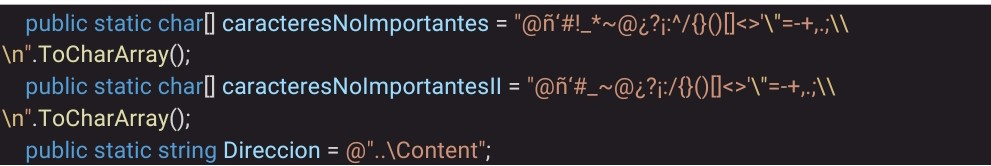
\includegraphics[width=\textwidth]{imagenes/1.jpg}
\end{figure}

Donde la dirección es el lugar donde están guardados los archivos en formato txt y los CaracteresNoImportantes serán los caracteres
a no tener en cuenta a la hora de leer los documentos.

\subsection{Class Leer Documentos}\label{sub:Leer Documentos}

En esta clase únicamente se leerán los archivos en formato txt que se encuentran en la carpeta Content y se guardaran los documentos
en un array de Documentos

\subsection{Class Documento}\label{sub:Documento}

En esta clase nos dedicaremos a crear variables de tipo Documento donde cada documento tendrá las siguientes propiedades

\begin{figure}[H]
    \centering
    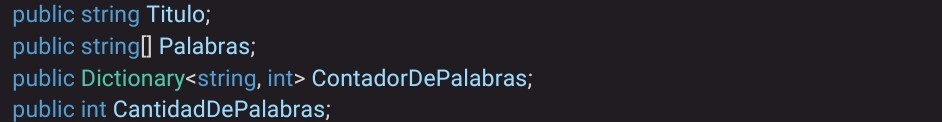
\includegraphics[width=\textwidth]{imagenes/2.jpg}
\end{figure}

El titulo será utilizado luego para mostrar los resultados de la consulta.

El resto de las propiedades serán necesarias para calcular el TFIDF.

Para crear un documento es necesario pasar como parámetros dos strings que serán el titulo y el texto.

Estos strings los obtendremos usando Clases y Metodos ya existentes en el lenguaje.

\subsection{Class Vector}\label{sub:Vector}

En esta clase crearemos variables de tipo vector que tendrán las siguientes propiedades

\begin{figure}[H]
    \centering
    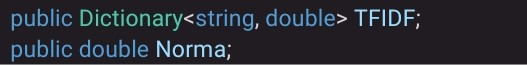
\includegraphics[width=0.7\textwidth]{imagenes/3.jpg}
\end{figure}

En esta clase el usuario puede observar que tenemos dos constructores 

El primero para crear vectores a través de un documento y el segundo creado especialmente para el string 
que entrara en la consulta.

Usando el primer constructor calcularemos primeramente el TF de cada palabra que se encuentra en cada Documento y lo 
guardaremos de momento en el diccionario llamado TFIDF, por supuesto no es eso lo que terminaremos guardando en este diccionario 
pero de momento queda precalculado ahí.
Tambien calcularemos la norma para cada documento utilizando el TFIDF que calcularemos en la Clase Cuerpo.

Para la query, o sea , el segundo constructor haremos algo similar calculando igualmente la norma y el TFIDF de cada palabra 
de la consulta.

En esta clase tenemos también métodos a utilizar como lo son:

\begin{figure}[H]
    \centering
    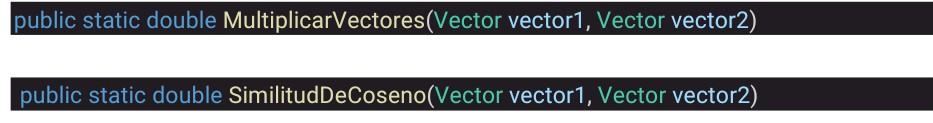
\includegraphics[width=\textwidth]{imagenes/4.jpg}
\end{figure}

El primero creado para ser utilizado en el segundo y hacer el código mas legible y organizado.

El método de similitud de coseno es utilizado luego en la clase Moogle para calcular la similitud entre un documento cualquiera y la query.

\subsection{Class Cuerpo}\label{sub:Cuerpo}

En esta clase crearemos un cuerpo de vectores donde tendremos las siguientes propiedades:

\begin{figure}[H]
    \centering
    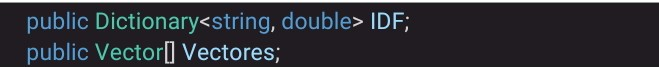
\includegraphics[width=\textwidth]{imagenes/5.jpg}
\end{figure}

Al constructor de esta clase es necesario pasarle como parámetro un array de variables de tipo Documento. 

Hemos decidido calcular el IDF aquí pues como es el mismo para cada palabra sin importar el documento , es común para todos los vectores.
Aquí crearemos un Vector para cada documento y calcularemos finalmente el TFIDF para cada palabra de cada uno de los documentos y lo guardaremos en Vector.TFIDF.

\subsection{Class Moogle}\label{sub:Moogle}

Tenemos un constructor en esta clase creado con el objetivo de calcular toda la información del TFIDF de los documentos contenidos en la carpeta Content y dejarlos 
guardados asi la búsqueda será mas rápida cuando se vuelva a ejecutar por segunda vez.

En esta clase tenemos métodos como :

\begin{figure}[H]
    \centering
    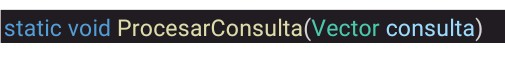
\includegraphics[width=0.6\textwidth]{imagenes/6.jpg}
\end{figure}

Donde procesaremos la consulta y calcularemos el TFIDF y la norma de esta haciendo uso de la clase Vector.

Otro metodo es:

\begin{figure}[H]
    \centering
    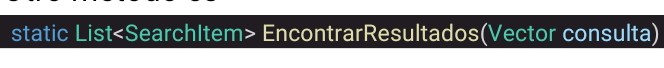
\includegraphics[width=0.9\textwidth]{imagenes/7.jpg}
\end{figure}

Donde llamaremos al método SimilitudDeCoseno contenido en la clase Vector y calcularemos la relevancia para cada documento con respecto a la query.
Tambien se ordenaran en una lista los documentos que tengan alguna relevancia y se realizara la búsqueda del snippet para dichos documentos.
Estos datos serán utilizados para crear variables de tipo SerchItem y por ultimo en el método.

\begin{figure}[H]
    \centering
    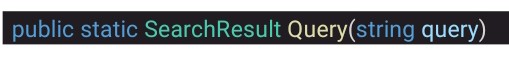
\includegraphics[width=0.7\textwidth]{imagenes/8.jpg}
\end{figure}

\section{TF-IDF}\label{sec:TF-IDF}

TF-IDF es una técnica utilizada en procesamiento de lenguaje natural para evaluar la relevancia de un término en un documento o corpus de textos. TF hace referencia a la frecuencia del 
término en el documento, mientras que IDF se refiere a la frecuencia inversa del término en el corpus.

TF (Term Frequency) mide la frecuencia con la que aparece un término en un documento específico. Cuanto mayor sea la frecuencia, más relevante se considera el término en ese documento.

IDF (Inverse Document Frequency) mide la importancia del término en el conjunto de documentos. Calcula la frecuencia inversa para los términos que aparecen en muchos documentos, lo que 
significa que si un término se repite en muchos documentos, su IDF será bajo y se  considerará menos relevante.

La combinación de TF y IDF es el resultado del cálculo del producto de TF y IDF, y es utilizado para clasificar y buscar documentos en función de su relevancia en relación con un término 
de búsqueda específico. Cuanto mayor sea el valor de TF-IDF de un término en un documento, más indicativo será su relevancia en ese documento específico.
Luego de conocido el TF-IDF de cada documento utilizaremos para establecer una comparación entre los Documentos y la consulta un método que es muy utilizado y conocido como el método de similitud de coseno.

\subsection{Similitud de Cosenos}\label{sub:SimilitudDeCoseno}

El método de similitud de coseno es una técnica utilizada en minería de textos y recuperación de información para determinar cuán similar es un documento o un conjunto de palabras en relación con otro documento o conjunto de palabras. 

Este método se basa en la idea de que la similitud entre dos vectores de características puede expresarse mediante el ángulo que forman en un espacio vectorial. En este caso, los vectores de características representan la frecuencia de las palabras en un documento (o conjunto de palabras).

Para calcular la similitud de coseno, primero se representan los documentos o conjuntos de palabras como vectores de características. Luego, se calcula el producto punto entre estos dos vectores y se divide por el producto de las magnitudes de los vectores.

El resultado de esta operación es un número entre -1 y 1, donde 1 indica una similitud perfecta, 0 indica que los documentos o conjuntos de palabras son completamente diferentes y -1 indica una similitud inversa.

En resumen, el método de similitud de coseno determina la similitud entre documentos o conjuntos de palabras al operar en el espacio vectorial de características y calcular el ángulo de coseno entre ellos.

\bibliography{bibliography}
\end{document}